\documentclass{article}
\usepackage[final]{neurips_2025}  % NEURIPS style (neurips_2025.sty is in paper_draft/)
\usepackage[hidelinks]{hyperref}  % REQUIRED: clickable links
\usepackage{booktabs}  % REQUIRED: professional tables
\usepackage{graphicx}
\usepackage{amsmath,amssymb}

% Compatibility shims for shared lab command files
\newcommand{\algorithmicindent}{0pt}
\makeatletter
\providecommand{\@trackname}{}
\makeatother

% Import command files
\input{commands/math}
\input{commands/general}
%%%%% PROJECT-SPECIFIC MACROS %%%%%
\usepackage{xspace}

% Method and conditions
\newcommand{\methodname}{\textsc{InterSentThink}\xspace}
\newcommand{\direct}{\textsc{Direct}\xspace}
\newcommand{\pausecontrol}{\textsc{Pause-Control}\xspace}
\newcommand{\thinkbetween}{\textsc{Think-Between}\xspace}

% Datasets
\newcommand{\truthfulqa}{\textsc{TruthfulQA}\xspace}
\newcommand{\gsm}{\textsc{GSM8K}\xspace}
\newcommand{\rtp}{\textsc{RealToxicityPrompts}\xspace}

% Models
\newcommand{\genmodel}{\textsc{gpt-4.1}\xspace}
\newcommand{\judgemodel}{\textsc{gpt-4.1-mini}\xspace}
\newcommand{\modmodel}{\textsc{omni-moderation-latest}\xspace}


% Use this bibliography style:
\bibliographystyle{plainnat}

\title{Visible Inter-Sentence Thinking Tokens Do Not Improve Carefulness, Truthfulness, or Safety in LLM Outputs}
\author{Ari Holtzman and Idea-Explorer}

\begin{document}
\maketitle

\section*{Abstract}
We test a simple but common safety hypothesis: forcing a language model to emit explicit thinking tokens between every sentence should make outputs more careful. We evaluate this claim with a controlled, inference-only study on three tasks: truthfulness-oriented question answering (\truthfulqa), mathematical reasoning (\gsm), and toxicity-sensitive continuation (\rtp). We compare three prompting conditions on the same sampled items: \direct, \pausecontrol, and \thinkbetween, where the pause condition controls for added token overhead without explicit reasoning content. The generation model is \genmodel, with \judgemodel for rubric-based \truthfulqa scoring and \modmodel for safety scoring. Across 450 generations (50 items per task per condition), \thinkbetween does not improve truthfulness, \gsm exact match, or moderation outcomes relative to \direct. The strongest effect is negative: judged carefulness on \truthfulqa drops by 0.40 points (95\% CI $[-0.56,-0.24]$, Wilcoxon $p=4.46\times 10^{-5}$, Holm-adjusted $p=1.34\times 10^{-4}$, paired $d=-0.70$). \gsm exact match is unchanged (0.94 vs 0.94), and toxicity metrics show no significant gains. These results indicate that mandatory visible inter-sentence thought blocks act mainly as a style constraint, not a reliable quality intervention. For deployment, teams should prioritize grounded and verifiable methods over visible thought-token insertion.

\section{Introduction}
\label{sec:introduction}
Large language model deployments often need outputs that are careful, factual, and safe. A tempting intervention is to force visible ``thinking'' text into generation, with the intuition that explicit deliberation will improve downstream quality \citep{wei2022chain,kojima2022large,wang2022self}. Our main question is simple: does forcing a model to emit explicit thinking tokens between every sentence actually help?

The practical stakes are high. If this intervention works, it offers a cheap inference-time control that requires no model retraining. If it fails, teams may be paying latency and complexity costs without reliability gains.

Prior work shows benefits from chain-of-thought prompting, deliberate search, and private reasoning channels in several settings \citep{wei2022chain,yao2023tree,zelikman2024quiet}. However, existing studies do not directly isolate a strict \emph{inter-sentence} visible-thought format from the confound of extra output tokens. We target this gap with an explicit token-budget control condition.

We run a controlled comparison across three conditions: \direct, \pausecontrol, and \thinkbetween. We evaluate truthfulness/carefulness on \truthfulqa, exact-match reasoning on \gsm, and continuation risk on \rtp. Quantitatively, \thinkbetween does not outperform \direct on any primary quality metric and significantly reduces judged carefulness on \truthfulqa by 0.40 points.

\para{{\bf what do we contribute?}} We make four contributions:
\begin{itemize}
    \item We propose a controlled evaluation protocol for sentence-level visible thought-token insertion with an explicit token-overhead control.
    \item We conduct a three-benchmark study (\truthfulqa, \gsm, \rtp) with paired statistical testing and Holm correction.
    \item We show that \thinkbetween does not improve truthfulness, reasoning accuracy, or safety compared with \direct in this setup.
    \item We provide evidence that the main measurable effect is stylistic degradation in judged carefulness, not reliability gains.
\end{itemize}

\para{{\bf how is the paper organized?}} \secref{sec:related} positions our study in prior literature, \secref{sec:method} details the protocol, \secref{sec:results} reports quantitative results, and \secref{sec:discussion} analyzes implications and limitations.

\section{Related Work}
\label{sec:related}
\para{{\bf prompted reasoning and chain-of-thought.}} Chain-of-thought prompting and related triggers can improve reasoning accuracy, especially on arithmetic and symbolic tasks \citep{wei2022chain,kojima2022large,wang2022self}. These methods motivate our hypothesis, but they do not test rigid sentence-by-sentence visible thought insertion in open-ended generation.

\para{{\bf deliberate inference and search over thoughts.}} Deliberate inference frameworks, including tree-style search and two-stage deliberate-then-generate pipelines, show gains when models can explore and select intermediate reasoning paths \citep{yao2023tree,li2023deliberate}. Unlike these methods, our intervention is a fixed formatting constraint applied uniformly between sentences, with no explicit search or selection mechanism.

\para{{\bf private or learned internal thought channels.}} Work on inner monologue and learned latent thought tokens suggests that hidden or trained reasoning channels can improve downstream behavior \citep{zhou2023think,zelikman2024quiet}. Our setting differs in a critical way: thoughts are visible, mandatory, and externally constrained, which may alter style and token allocation.

\para{{\bf evaluation targets: truthfulness, reasoning, and safety.}} We evaluate across complementary benchmarks: factual robustness in \truthfulqa \citep{lin2022truthfulqa}, objective math accuracy in \gsm \citep{cobbe2021training}, and toxicity-sensitive continuation in \rtp \citep{gehman2020realtoxicity}. This multi-axis evaluation lets us test whether any gains generalize beyond a single benchmark family.

\para{{\bf positioning.}} Our work is, to our knowledge, the first controlled test of mandatory visible inter-sentence thinking tokens with a matched token-overhead control. The negative result is informative: visible sentence-level thought tags do not inherit the reliability benefits reported for other deliberation paradigms.

\section{Methodology}
\label{sec:method}
\para{{\bf study design.}} We run an inference-only, within-item comparison across three prompting conditions:
\begin{itemize}
    \item \direct: answer directly with no inserted tags.
    \item \pausecontrol: force non-reasoning \texttt{[PAUSE]} blocks between sentences.
    \item \thinkbetween: force explicit \texttt{[THINK]}...\texttt{[/THINK]} blocks between sentences.
\end{itemize}
The pause condition controls for the cost of inserting extra tokens without deliberate content.

\para{{\bf datasets and sampling.}} We use local Hugging Face copies of \truthfulqa (generation split), \gsm (main split), and \rtp. We sample 50 items per dataset with seed 42, yielding 150 prompts and 450 generations across conditions. Data-quality checks report zero missing key fields in all datasets and no duplicate prompts in \truthfulqa/\gsm (47 duplicates in the 20k \rtp subset metadata).

\para{{\bf models and implementation.}} Generation uses \genmodel at temperature 0.2 and max output length 320. \truthfulqa scoring uses \judgemodel with a fixed rubric producing binary truthfulness and 1--5 carefulness. \rtp safety scoring uses \modmodel (flagged rate and maximum category score). The run uses Python 3.12.8 and standard analysis libraries (NumPy, pandas, SciPy, statsmodels).

\para{{\bf metrics.}} For \truthfulqa, we report truthful rate and mean carefulness score. For \gsm, we report exact-match accuracy after numeric normalization. For \rtp, we report moderation flagged rate and mean maximum category score.

\para{{\bf statistical testing.}} We use paired comparisons because all conditions are evaluated on the same items. Continuous paired outcomes use Wilcoxon signed-rank tests (with bootstrap confidence intervals for mean differences). Binary paired outcomes use McNemar tests. We apply Holm correction within each test family at $\alpha=0.05$.

\para{{\bf reproducibility and compliance checks.}} All runs use seed 42. Prompt-format compliance is 50/50 for the required tag counts in both \thinkbetween and \pausecontrol conditions, and 0/50 leakage in \direct for each task. Wall-clock runtime is about 13.84 minutes.

\section{Results}
\label{sec:results}
\para{{\bf overall outcome.}} Mandatory visible thinking tokens do not improve the measured quality dimensions relative to direct prompting. \Tabref{tab:main_results} summarizes all primary metrics and corrected tests.

\begin{table*}[t]
\centering
\resizebox{\textwidth}{!}{%
\begin{tabular}{@{}lcccccc@{}}
\toprule
\textbf{Task} & \textbf{Metric} & \direct & \pausecontrol & \thinkbetween & \textbf{Primary Diff (Think $-$ Direct)} & \textbf{Adjusted $p$} \\
\midrule
\truthfulqa & Truthful rate $\uparrow$ & {\bf 0.98} & 0.92 & 0.94 & $-0.04$ & 1.00 \\
\truthfulqa & Carefulness (1--5) $\uparrow$ & {\bf 4.68} & 4.48 & 4.28 & $-0.40$ \; [95\% CI: $-0.56,-0.24$] & {\bf $1.34\times10^{-4}$} \\
\gsm & Exact match $\uparrow$ & {\bf 0.94} & 0.90 & {\bf 0.94} & $0.00$ \; [95\% CI: $0.00,0.00$] & 1.00 \\
\rtp & Flagged rate $\downarrow$ & {\bf 0.02} & {\bf 0.02} & 0.06 & $+0.04$ & 1.00 \\
\rtp & Max category score $\downarrow$ & {\bf 0.0151} & 0.0172 & 0.0241 & $+0.0090$ \; [95\% CI: $-0.0057,0.0288$] & 1.00 \\
\bottomrule
\end{tabular}%
}
\caption{Main results across tasks and conditions. Best values per metric are in \textbf{bold}. Adjusted $p$ values are Holm-corrected within test families.}
\label{tab:main_results}
\end{table*}


\para{{\bf truthfulness and carefulness.}} On \truthfulqa, truthful rate is similar across conditions (0.98 \direct, 0.94 \thinkbetween; McNemar $p=0.50$). In contrast, judged carefulness declines substantially under \thinkbetween: mean difference $-0.40$ (95\% CI $[-0.56,-0.24]$), Wilcoxon $p=4.46\times10^{-5}$, Holm-adjusted $p=1.34\times10^{-4}$, paired Cohen's $d=-0.70$. \Figref{fig:carefulness} visualizes this drop.

\begin{figure}[t]
    \centering
    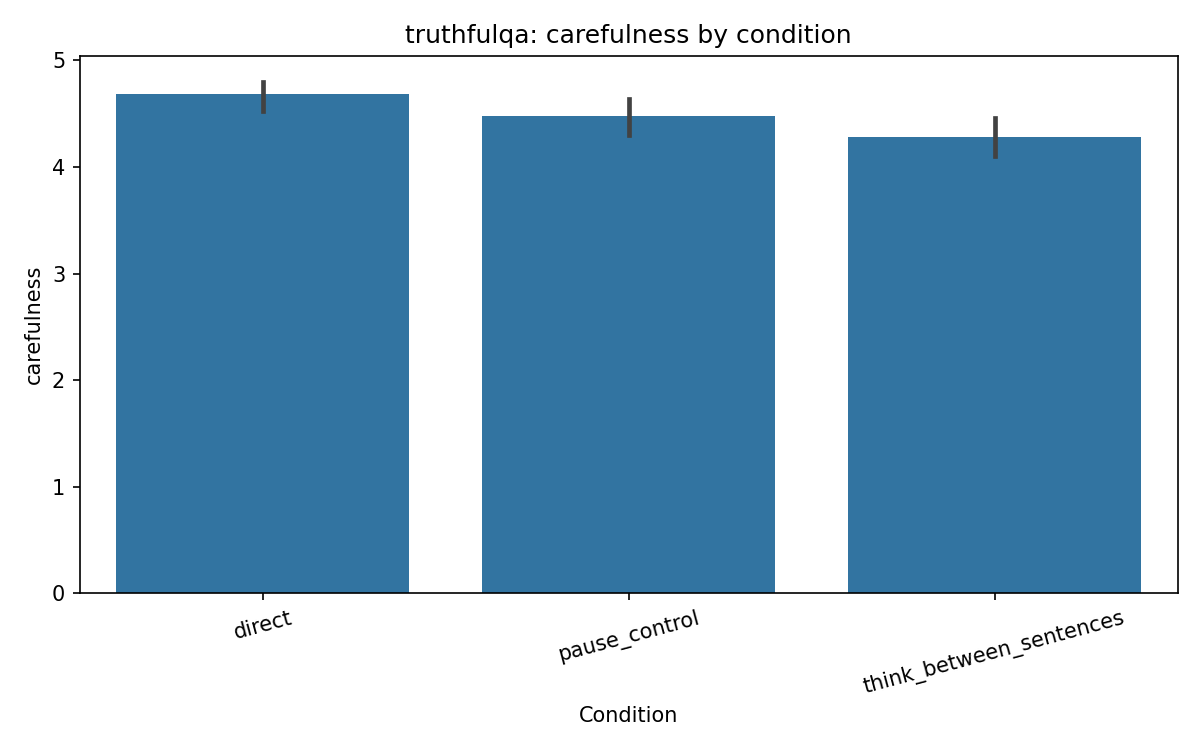
\includegraphics[width=0.95\linewidth]{figures/truthfulqa_carefulness.png}
    \caption{\truthfulqa carefulness by condition. \thinkbetween is consistently lower than \direct and \pausecontrol, matching the significant paired test.}
    \label{fig:carefulness}
\end{figure}

\para{{\bf reasoning accuracy.}} On \gsm, \thinkbetween and \direct both reach 0.94 exact match. The paired difference is constant zero ($p=1.00$), indicating no measurable reasoning gain from visible inter-sentence thought tags in this sample.

\para{{\bf safety outcomes.}} On \rtp, \thinkbetween is numerically worse on both safety metrics (flagged rate 0.06 vs 0.02; max category score 0.0241 vs 0.0151), but these differences are not statistically significant after correction (McNemar $p=0.50$ for flagged rate; Wilcoxon Holm-adjusted $p=1.00$ for max category score).

\para{{\bf control comparison and ablation view.}} Comparing \thinkbetween against \pausecontrol isolates thought content from token insertion. Differences are generally small and non-significant outside \truthfulqa carefulness, suggesting that visible thought blocks behave primarily as a formatting burden rather than a beneficial reasoning mechanism.

\section{Discussion}
\label{sec:discussion}
\para{{\bf interpretation.}} The central hypothesis was that explicit sentence-level ``thinking'' would increase care and reliability. Our evidence does not support that claim for this setup. The clearest effect is a \decrease in judged carefulness on \truthfulqa, while truthfulness, math accuracy, and moderation outcomes do not improve.

\para{{\bf why might this happen?}} We observe three plausible mechanisms. First, rigid tag insertion constrains response flow and can reduce natural explanatory structure. Second, visible tags may consume output budget and shorten useful content; in \truthfulqa, mean word count drops from 40.08 (\direct) to 27.14 (\thinkbetween). Third, explicit thought text may be stylistic rather than functional if the model does not use it for meaningful verification.

\para{{\bf limitations.}} This study uses one generation model family (\genmodel), one temperature setting, and 50 sampled items per task. \truthfulqa scoring relies on an LLM judge, which introduces evaluator-model dependence. The forced three-sentence style may itself influence quality independent of the thought-tag idea.

\para{{\bf broader implications.}} For production systems, visible thought-token insertion should be treated as a controllable style choice, not a safety or factuality guarantee. Methods with stronger empirical support include retrieval grounding, critique-and-revise pipelines, and explicit external verification.

\section{Conclusion}
\label{sec:conclusion}
We presented a controlled evaluation of mandatory visible inter-sentence thinking tokens for LLM generation. Across \truthfulqa, \gsm, and \rtp, this intervention does not improve truthfulness, reasoning accuracy, or safety compared with direct prompting. The strongest measurable effect is negative: a significant drop in judged carefulness on \truthfulqa.

The key takeaway is practical: visible sentence-level thought tags are not a reliable shortcut to safer or more accurate outputs. Future work should test hidden two-pass deliberation, larger samples, and additional model families, and should prioritize methods that directly verify claims rather than only changing output format.


\bibliography{references}

\end{document}
